\documentclass[10pt,t]{beamer}
\usetheme{Heverlee}

\usepackage{tikz-cd}

\newcommand{\F}{\mathbb F}


%%% QUICK OPTIONS:
% (A) Math font without serifs, enable line below to make math serif:
    \usefonttheme[onlymath]{serif}

% (B) Re-define primary colour by adjusting the RGB values
    %\definecolor{pblue}	{RGB}{206,125,66}

% (C) Title page graphic (optional) --- this is not for the background image, see \usebackgroundtemplate to change that ---
    %\titlegraphic{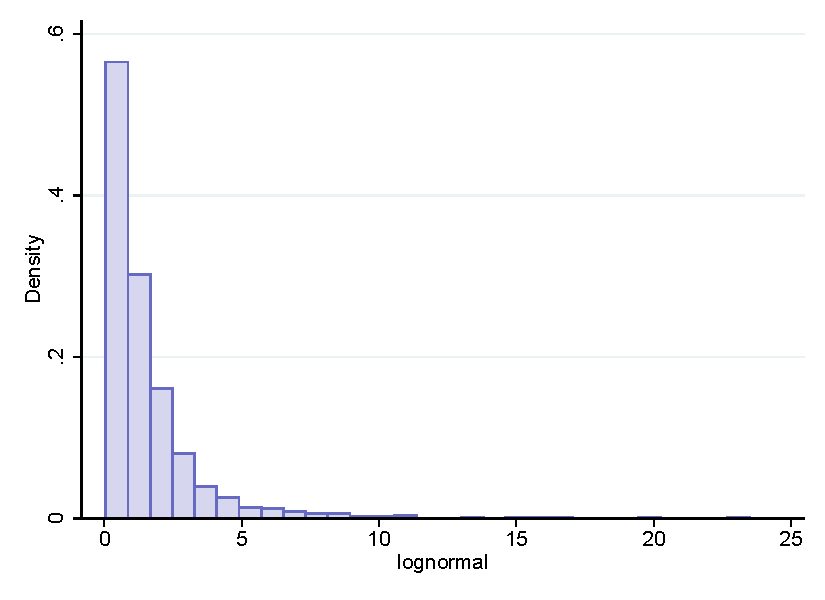
\includegraphics[height=2.7cm]{example_figure.pdf}}

% (D) Add logo to bottom right-corner (optional)
    \logo{\includegraphics[height=0.7cm]{icosahedron-src.pdf}\hspace{12pt}\vspace{-6pt}} 

% (E) Choose one (or none) of these lines to add footline bar on all frames
    %\setbeamertemplate{footline}[infoline]  % author, title, insitute
    %\setbeamertemplate{footline}[navigation] % dots swhowing progress
    %\setbeamertemplate{footline}[navsym] % navigation symbols

% (F) Widescreen 16:9 ratio
    %\usepackage[orientation=landscape,size=custom,width=16,height=9,scale=0.45,debug]{beamerposter} 



%%% TITLE PAGE INFO:

\title[clesto]{Chain level Steenrod operations}
\subtitle{Theoretical and computational aspects}
\author[ammedmar]{Anibal M. Medina-Mardones}
\institute{Max Planck Institute for Mathematics in Bonn}
\date{January 2021}

\begin{document}
% Title page

{
% Change image, or delete this line to remove background image
\usebackgroundtemplate{ \parbox[b][\paperheight][b]{\paperwidth}{\centering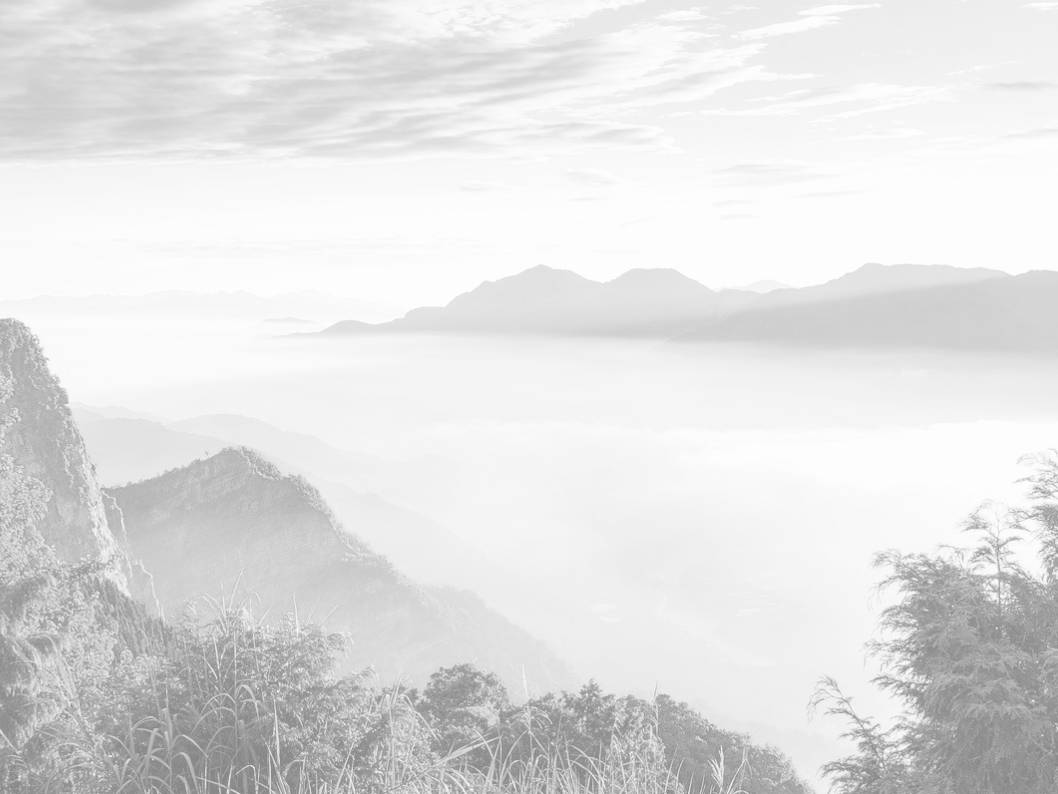
\includegraphics[width=\paperwidth]{bg_alishan.jpg}}} 
 %   abudhabi      cherry      forest      river
 %   alishan       chobe       leuven      sanfancisco
 %   blueprint     columns     library     uyuni
 %   bokeh         flowers     newyork     winter

% \setbeamercolor{background canvas}{bg=lgray}  % make background light gray

\begin{frame}[plain,noframenumbering]
    \titlepage
\end{frame}
}

% Table of contents slide
\begin{frame}{Outline}
	\vskip 2mm
	\hfill	{\large \parbox{.95\textwidth}{\tableofcontents[hideothersubsections]}}
\end{frame}

%%  SECTION 1

\section{History and motivation} \label{sec: history and motivation}

\begin{frame}[fragile]{Diagonal and cup product}
	The diagonal map of spaces
	\begin{equation*}
	\begin{tikzcd}[row sep = tiny]
	X \arrow[r, "D"] & X \times X \\
	x \arrow[r, |->]& (x, x)
	\end{tikzcd}
	\end{equation*}
	induces a product in cohomology with field coefficients
	\begin{equation*}
	\begin{tikzcd}[row sep = tiny]
	\smallsmile \colon &[-20pt] H^\bullet(X) \otimes H^\bullet(X) \arrow[r, "\cong"] &[-5pt] H^\bullet(X \times X) \arrow[r, "H^\bullet(D)"] &[5pt] H^\bullet(X), \\
	\end{tikzcd}
	\end{equation*}
	
	\pause
	
	which is (graded) commutative, since the diagonal is invariant under the transposition
	\begin{equation*}
	\begin{tikzcd}[row sep = tiny]
	X \times X \arrow[r, "T"] & X \times X \\
	(x, y) \arrow[r, |->]& (y, x).
	\end{tikzcd}
	\end{equation*}
	
	\vspace*{5pt} \pause
	
	\textcolor{pblue}{How about integer coefficients?}
\end{frame}


\begin{frame}[fragile]{Diagonal and cup product}
	During the mid 1930's Alexander, Kolmogorov, \v{C}ech and Whitney defined the cup product dualizing a simplicial chain approximation to the diagonal
	\begin{equation*}
	\begin{tikzcd}[%
	,row sep = 0ex
	,/tikz/column 1/.append style={anchor=base east}
	,/tikz/column 2/.append style={anchor=base west}
	]
	C_\bullet \arrow[r, "\Delta"] & C_\bullet \otimes C_\bullet \\
	{[0, \dots, n]} \arrow[r, |->] & \sum_{i=0}^{n} {[0, \dots, i] \otimes [i, \dots, n]}.
	\end{tikzcd}
	\end{equation*}

	\pause \vspace*{10pt}

	It is not invariant under the transposition
	\begin{equation*}
	\begin{tikzcd}[row sep = tiny]
	C_\bullet \otimes C_\bullet \arrow[r, "T"] & C_\bullet \otimes C_\bullet \\
	a \otimes b \arrow[r, |->]& (-1)^{|a||b|} b \otimes a.
	\end{tikzcd}
	\end{equation*}
	
	\vspace*{10pt}\pause
	
	\textcolor{pblue}{Can it be made to be?}
	
	


\end{frame}


\begin{frame}{Steenrod's obstructions to commutativity}
	In 1947, Steenrod published his seminal paper introducing the square operations through an effective construction of homotopies correcting the lack of symmetry of $\Delta$ (denoted $\Delta_0 = $ from now on).

	\vspace*{15pt} \pause

	\textcolor{pblue}{Recall:} The set of linear maps between chain complexes is a chain complex.
	Chain maps $\sim$ $0$-cycles, chain homotopies $\sim$ $1$-boundaries.

	\vspace*{15pt}\pause

	\textcolor{pblue}{Notice:} The chain complex
	\begin{equation*} \label{eq: complex of maps to the tensor product}
	Hom\left(C_\bullet, C_\bullet^{\otimes 2}  \right)
	\end{equation*}
	has a left $\Sigma_2$-action induced from $T$, and there is a $0$-cycle of interest:
	\begin{equation*}
	\Delta_0 - T \Delta_0.
	\end{equation*}
\end{frame}


\begin{frame}{Steenrod's obstructions to commutativity}
	The cup-$1$ coproduct
	\begin{equation*}
	\Delta_1 [0, \dots, n] = \sum_{i<j} \pm [0, \dots, i, j, \dots, n] \otimes [i, \dots, j]
	\end{equation*}
	is boundary killing this cycle. But is itself \textbf{not symmetric}.
	
	\vspace*{10pt} \pause
	
	Steenrod gave formulae for higher corrections, the cup-$i$ coproducts:
	\begin{equation*}
	\partial (\Delta_{i+1}) = \Delta_i - (-1)^i T \Delta_i.
	\end{equation*}
	
	\vspace*{0pt}\pause
	
	More abstractly, if
	\begin{equation*}
	W(2) \quad = \quad \mathbb Z[\Sigma_2] \stackrel{\ 1-T}{\longleftarrow} \mathbb Z[\Sigma_2] \stackrel{\ 1+T}{\longleftarrow} \mathbb Z[\Sigma_2] \stackrel{\ 1-T}{\longleftarrow} \cdots
	\end{equation*}
	is the minimal free resolution of $\mathbb Z$ as a $\mathbb Z[\Sigma_2]$-module, \pause he effectively constructed an equivariant chain map
	\begin{equation*}
	W(2) \otimes C_\bullet \to C_\bullet^{\otimes 2}.
	\end{equation*}
\end{frame}
	

\begin{frame}[fragile]{Steenrod obstructions to commutativity}
	Using the $\F_2$-duality functor and passing to fix points, we have a chain map 
	\begin{equation*}
	\begin{tikzcd}
	Hom\left(C_\bullet \otimes C_\bullet, \F_2 \right)^{\Sigma_2} \arrow[r] &
	Hom\left(W(2) \otimes C_\bullet, \F_2 \right)^{\Sigma_2}
	\end{tikzcd}
	\end{equation*}
\end{frame}
%%%%%%%%%%%%%
\begin{frame}[fragile]{Steenrod obstructions to commutativity}
	Using the $\F_2$-duality functor and passing to fix points, we have a chain map 
	\begin{equation*}
	\begin{tikzcd}
	Hom\left(C_\bullet \otimes C_\bullet, \F_2 \right)^{\Sigma_2} \arrow[r] &
	Hom\left(W(2) \otimes C_\bullet, \F_2 \right)^{\Sigma_2} \arrow[d] \\
	\left(C^\bullet \otimes C^\bullet\right)^{\Sigma_2} \arrow[u] &
	Hom\left(W(2)_{\Sigma_2} \otimes C_\bullet, \F_2 \right)
	\end{tikzcd}
	\end{equation*}
\end{frame}
%%%%%%%%%%%%%
\begin{frame}[fragile]{Steenrod obstructions to commutativity}
	Using the $\F_2$-duality functor and passing to fix points, we have a chain map 
	\begin{equation*}
	\begin{tikzcd}
	Hom\left(C_\bullet \otimes C_\bullet, \F_2 \right)^{\Sigma_2} \arrow[r] &
	Hom\left(W(2) \otimes C_\bullet, \F_2 \right)^{\Sigma_2} \arrow[d] \\
	\left(C^\bullet \otimes C^\bullet\right)^{\Sigma_2} \arrow[u]&
	Hom\left(W(2)_{\Sigma_2} \otimes C_\bullet, \F_2 \right) \arrow[d] \\
	C^\bullet \arrow[u, "Double"] \arrow[r, dashed]&
	Hom\left(W(2)_{\Sigma_2}, C^\bullet\right) \\
	\end{tikzcd}
	\end{equation*}
	
	\vspace*{-20pt}\pause
	
	By adjuntion, we obtain a chain map
	\vspace*{-2pt}
	\begin{equation*}
	\begin{tikzcd}[row sep=tiny, column sep = tiny]
	C^\bullet \otimes W(2)_{\Sigma_2} \arrow[r] &[-10pt] C^\bullet \\
	\alpha \otimes e_i \arrow[r, |->] & (\alpha \otimes \alpha)\Delta_i(-)
	\end{tikzcd}
	\end{equation*}
	
	\vspace*{-5pt}\pause
	
	\textcolor{pblue}{Take away:} The mod-2 homology of $\Sigma_2$ defines operations on the mod-2 cohomology of spaces.
\end{frame}


\begin{frame}[fragile]{Steenrod obstructions to commutativity}
	The Steenrod squares are defined by reindexing the previous map
	\begin{equation*}
	\begin{tikzcd}[row sep=tiny, column sep=tiny]
	Sq^k \colon H^{-n} \arrow[r] & H^{-n-k} \\
	\phantom{Sq^k \colon}{[\alpha]} \arrow[r, |->] & {\left[(\alpha \otimes \alpha)\Delta_{n-k}(-) \right]}
	\end{tikzcd}
	\end{equation*}
	Their importance in stable homotopy theory is hard to overstate.
	
	\pause \vspace{\baselineskip}
	
	By construction, their non-triviality is an obstruction to a \textbf{commutative} product of cocycles.
	
	\pause \vspace{\baselineskip}
	
	The relevance of the cup-$i$ coproducts $\Delta_i$ goes beyond their use defining the $Sq^k$ operations.
		
\end{frame}


\begin{frame}{The relevance of chain level Steenrod squares}
	The explicit formulae for the cup-$i$ (co)products	
	\begin{itemize}
		\item Are used in the definition of action functionals in lattice models in quantum field theory (Kapustin, Thorngren), \pause
		\item Are used in persistence (co)homology to extract finner information of data sets (MM--Tauzin), \pause
		\item Define the nerve of higher categories (MM), \pause
		\item Can be axiomatically characterized in analogy to the axioms for Steenrod square (MM), \pause
		\item Are used to construct effective chain approximation to spin bordism (Brumfiel--Morgan), \pause
		\item Are used to construct mod-2 operations on Khovanov homology (Cantero-Moran), \pause
		\item Can be used to construct cochains enforcing the Cartan (MM) and Adem (Brumfiel--MM--Morgan) relations,
		\item \ $\cdots$
	\end{itemize}
\end{frame}


\begin{frame}{Higher diagonals and the homology of $\Sigma_p$}
	What do we need to generalize the construction of Steenrod squares?
	
	\pause \vspace{10pt}
	
	\begin{enumerate}
		\item Construct $\Sigma_p$-equivariant maps
		\begin{equation*}
		E\Sigma_p \otimes C_\bullet \to C_\bullet^{\otimes p}
		\end{equation*}
		for $E\Sigma_p$ a resolution of $\mathbb Z$ by free $\mathbb Z[\Sigma_p]$-modules.
		\vspace*{10pt} \pause
		\item Identify chains in $E\Sigma_p$ whose orbits in $(E\Sigma_p)_{\Sigma_p} = B\Sigma_p$ represent mod-$p$ homology classes.
	\end{enumerate}

	\vspace*{10pt}\pause

	The first step is systematized by the use of operads, which we describe next, and the second is simplified by the group theoretical fact that the mop-$p$ homology of $\Sigma_p$ is detected by any cyclic subgroup of order $p$.
\end{frame}


\section{Operads and their algebras}

\begin{frame}[fragile]{Canonical example}
	Let $C$ be a chain complex, Consider the set
	\begin{equation*}
	End^C = \left\{Hom(C, C^{\otimes r})\right\}_{r \geq 1}.
	\end{equation*}
	
	\pause
	
	Is equipped the structure of an operad:
	\begin{itemize}
		\item A left action of $\Sigma_r$ on $End^C(r)$,
		\item Composition chain maps
		\begin{equation*}
		\begin{tikzcd}[column sep=small, row sep=tiny]
		\circ_i \colon &[-10pt] End^C(r) \otimes End^C(s) \arrow[r] & End^C(r+s-1) \\
		& f \otimes g \arrow[r, |->] & (1 \otimes \cdots \otimes g \otimes \cdots \otimes 1) \circ f 
		\end{tikzcd}
		\end{equation*}
	\end{itemize}
	satisfying forms of equivariance, associativity, and unitality.
	
	\pause \vspace*{10pt}
	
	\textcolor{pblue}{Slogan:} Abstract groups are to automorphisms of complexes like operads are to these coendomorphism examples.
\end{frame}


\begin{frame}[fragile]{Coalgebras}
	Let $\mathcal O$ be an operad, a coalgebra on $C$ is a structure preserving morphism
	\begin{equation*}
	\mathcal O \to End^C.
	\end{equation*}
	This compatibly parameterizes maps $C \to C^{\otimes r}$ by elements in $\mathcal O(r)$.
	
	\pause \vspace*{10pt}
	
	Compare with Steenrod's
	\vspace*{-2pt}
	\begin{equation*}
	\begin{tikzcd}[%
	row sep=tiny,
	column sep = small,
	,row sep = 0ex
	,/tikz/column 1/.append style={anchor=base east}
	,/tikz/column 2/.append style={anchor=base west}
	]
	W(2) \arrow[r] & Hom\left(C_\bullet, C_\bullet^{\otimes 2}\right) \\
	e_i \arrow[r, |->] & \Delta_i
	\end{tikzcd}
	\end{equation*}
	
	\pause
	We want free resolutions at every prime arity.
	
	\begin{definition}
		An $E_\infty$-operad $\mathcal R$ is one with each $\mathcal R(r)$ a resolution of $\mathbb Z$ by free $\mathbb Z[\Sigma_r]$-modules
	\end{definition}
	
\end{frame}

\section{Examples}

\section*{References}

\begin{frame}%[allowframebreaks]
	\frametitle{References}
	\nocite{whitney1935history}
	\bibliographystyle{amsalpha}
	\bibliography{biblio.bib}
\end{frame}


\end{document}
